\documentclass{article}
\usepackage{parskip}
\usepackage[letterpaper, portrait, margin=1.5in]{geometry}
\usepackage{graphicx}
\usepackage{subfigure}

\graphicspath{ {./images/} }

\usepackage{hyperref}
\hypersetup{
    colorlinks=true,
    linkcolor=blue,
    filecolor=magenta,      
    urlcolor=cyan,
}

\title{CS315 Algorithms Project Report: Pitch Shifting}
\date{2017-12-7}
\author{Grant Cox}

\begin{document}
	\pagenumbering{gobble}
	\maketitle
	\pagenumbering{arabic}

\section{Abstract}

Pitch correction, or "pitch shifting" is a method used frequently in digital signals processing (DSP) and audio processing. This is particularly useful for sound recordings, where a pitch shift is executed over an audio file, raising or lowering it a predefined number of keys. The algorithm detailed in this report reliably produces shifted signals as the user requests.

\section{Introduction}
Pitch shifting takes a wave and raises or lowers the frequency at least one semitone. In music theory, a semitone is one half step away from the current note. For example, if the original wave is a song in the key of C, the pitch shift could raise all the frequencies in the wave such that it is transformed to the same recording in C\#, or lowered such that the recording is in B. This algorithm can go beyond single semitones, raising or lowering the pitch a maximum of one octave (12 semitones).

The algorithm requires a Short Time Fourier Transform (STFT) and post-processing to accurately change the pitch. The goal is to shift the pitch up or down, while maintaining the length of the signal (in seconds). In addition, the pitch shifting algorithm should be able to execute a zero shift, where it would return the same wave as the original. To understand the pitch shifting algorithm, you must have an understanding of the FFT and how it is useful for pitch shifting, among countless other applications.

\section{Methods}
\subsection{Software}
This implementation of the pitch shifting algorithm was written in C++11 and compiled with  g++ on a machine running Ubuntu 16.04. The following libraries and files were referenced in the source code: smbPitchShift.cpp, armadillo, and AudioFile. Matlab R2017a was used for the analysis and plotting of the shifted signals. Audacity was used generate signals and perform analysis. VLC was used to play soundfiles.
\subsection{Algorithms}
\subsubsection{Fourier Transform}
The Discrete Fourier Transform (DFT) is an integral part of the pitch shifting process. The DFT builds upon Fourier's proof that any periodic waveform can be represented by the sum of an infinite set of sine waves. In signals processing, however, the process must be discrete and computable. The DFT algorithm takes a function (signal) that exists in the time domain and represents it in the frequency domain. In the time domain, a signal is represented with the time on the x-axis and the amplitude on the y axis. In the frequency domain, a set of frequencies are represented on the x-axis with the amplitude and phase at each frequency represented on the y axis.

The DFT requires $\theta(n^2)$ time to compute. The result of a DFT is an array (\textit{X}) with \textit{N} frequency bins, where \textit{N} is the same number of samples that were in the original signal (\textit{x}). \textit{X} \textbf{must} be the same size as \textit{x}. Each frequency bin holds a complex number with a magnitude and phase and should correspond to a frequency. Each frequency bin does not necessarily correspond to one single integer frequency, but often holds a very small range of frequencies. The true frequency of a frequency bin is calculated by the following equation, where $f_n$ is the true frequency, \textit{n} is the $n^{th}$ bin, \textit{s} is the sampling frequency of the original signal, and \textit{N} is the number of samples.

\begin{equation}
f_n = n * \frac{s}{N}
\end{equation}

The equation for the DFT is outlined below, where \textit{$X_k$} is the \textit{$k^{th}$} frequency bin, \textit{$x_n$} is the $n^{th}$ sample, \textit{j} is $\sqrt{-1}$, and \textit{N} is the number of samples:

\begin{equation}
X_k = \sum_{n=0}^{N-1} x_n * e^{\frac{-j*2\pi*k*n}{N}}
\end{equation}

Using this algorithm, frequency data can be easily obtained and measured over the signal input to the algorithm. The prominence of a frequency is quickly accessible inside X.

For pitch shifting purposes, the trivial idea would be to take the DFT of the entire signal and shift each element of X over the appropriate number of bins, then convert back to the time domain. However, the results will be quite messy. The problem arises when the signal is not a constant frequency, and vitrually all recorded signals in the real world are not. Taking the DFT of the entire signal and shifting simply  will not work. For example, there are plenty of occurrences of waves around 500Hz in the recording of ''I Don’t Wanna Know'' by Fleetwood Mac. If we take the DFT of the whole recording so that we can pitch shift, then all of the instances of 500Hz will be averaged out and be indistinguishable from one another. Thus, a different method must be used.
	
\subsubsection{Short Time Fourier Transform}
The method of choice for this algorithm is to iterate over \textit{x}, taking very small groups of samples, also known as “frames.” If the windows are small enough, the signal captured inside the window appears to be relatively constant over that time period. Splitting the data into more manageable chunks with a divide-and-conquer method is an effective way to pitch shift. For that reason, the algorithm relies on the Short Time Fourier Transform (STFT), where the signal is split into small chunks that are individually transformed. These frames are transformed using the Fast Fourier Transform (FFT), which takes advantage of the symmetry of the DFT and reduces the computational time to $O(\frac{N}{2}log_2(n))$.

When performing the STFT, there is only a slim chance that the period of the wave will line up perfectly within the frame. If this were the case, the frame's perspective would see that the wave is perfectly in phase with it (the frame starts and stops at zero amplitude on the wave). It is much more likely that the wave will appear out of phase with the window, as seen below. From the frame's point of view, the wave looks to start before the frame starts.

\begin{figure}[h]
\hfill
\subfigure[No Phase]{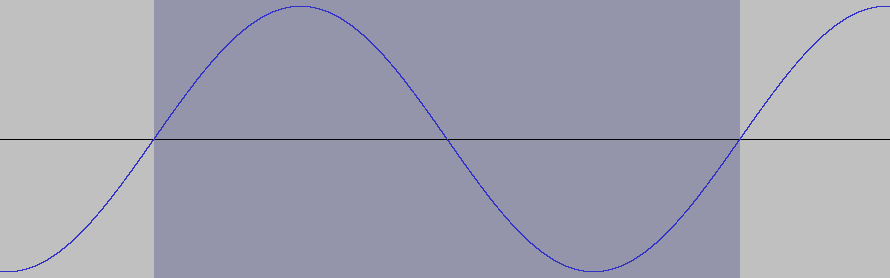
\includegraphics[width=.49\linewidth]{perfectWindow.png}}
\hfill
\subfigure[Phased]{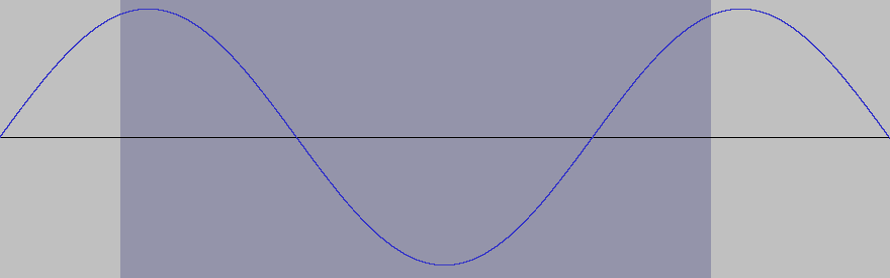
\includegraphics[width=.49\linewidth]{imperfectWindow.png}}
\hfill
\end{figure}

The method to solve this problem is to overlap the STFT frames with an integer overlapping factor (typically between 2 and 8), where the samples are transformed multiple times. The frame moves along at a proportion of the frame width decided by the STFT.

Using the properties of the STFT and frame overlapping, the problem with phasing out of the frame can be fixed. The magnitude shows how prominent the signal is in the frequency bin, the frequency shows what frequency bin range it fits into, and the phase tells the offset from the frequency bin.  Using these, the true frequency of the wave in the frame is possible to compute with the following equation, where \textit{R} is the sample rate, \textit{D} is the DFT frame size, \textit{i} is the $i^{th}$ bin, \textit{$p_i$} is the phase offset at bin \textit{i}, and \textit{s} is the overlap factor:

\begin{equation}
f_i = \frac{R}{D} * (i + \frac{p_i * s}{2\pi})
\end{equation}
	
\subsubsection{Shifting}
Once the program has iterated over all possible frames, the algorithm has amassed an array of true frequencies of all STFT frames. All that is required is to put the frequencies in the shifted partial frame where they belong. That multiplying factor \textit{f} is defined by the equation below, with \textit{s} as the number of semitones to raise or lower the recording:

\begin{equation}
f = 2^{s/12}
\end{equation} 

Finally, the shifted array can be inverse transformed back into the time domain, and there will be the outputted signal. The inverse transform is similar to the DFT, and is written as such:
\begin{equation}
x_n = \frac{1}{N} \sum_{k=0}^{N-1} X_k * e^{\frac{j*2\pi*k*n}{N}}
\end{equation}
This concludes the steps of the pitch shifting algorithm.

\section{Results}
Two sample files were passed through the program for this report. First, a sine wave was generated with Audacity, and output to a .wav file. This file was passed into the program twice, once shifting it down 1 semitone, and once shifting it up 2 semitones. Using matlab, the FFT of the three .wav files was taken and plotted on the graph below, which shows the shifts moving away from the original frequency.

\begin{figure}[h]
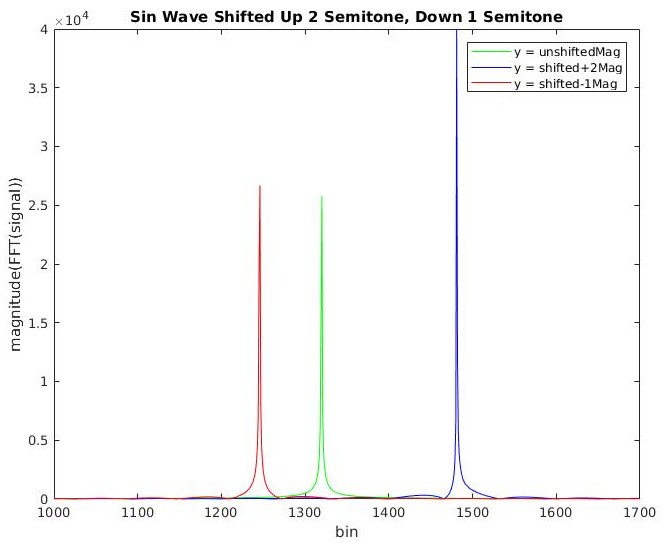
\includegraphics[width=.7\textwidth]{allsine.jpg}
\centering
\end{figure}

In addition, the clip from the song ''I Don’t Wanna Know'' by Fleetwood Mac was passed into the program. The same procedure was performed over this file, raising it 3 semitones. Using Matlab, the results were plotted, with a zoomed image for clarity.

\begin{figure}[h]
\hfill
\subfigure[Full View]{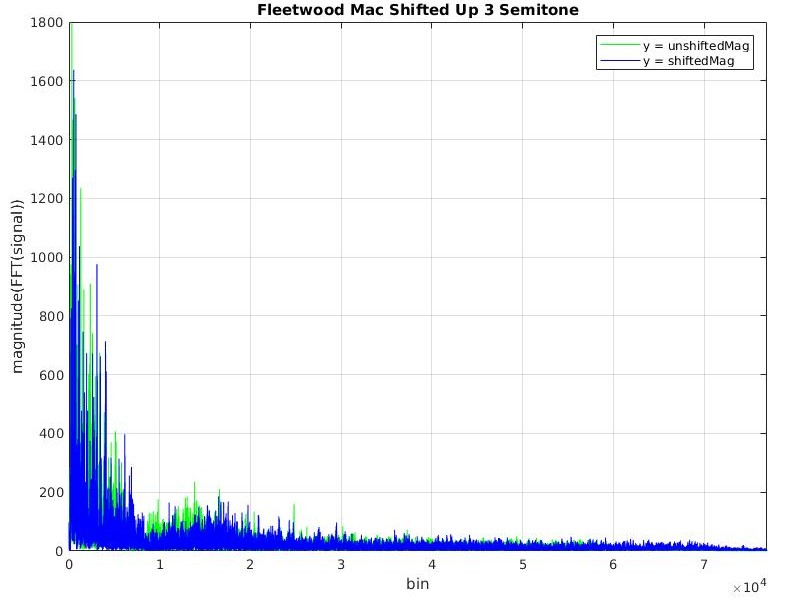
\includegraphics[width=.49\linewidth]{fleet+3.jpg}}
\hfill
\subfigure[Zoomed]{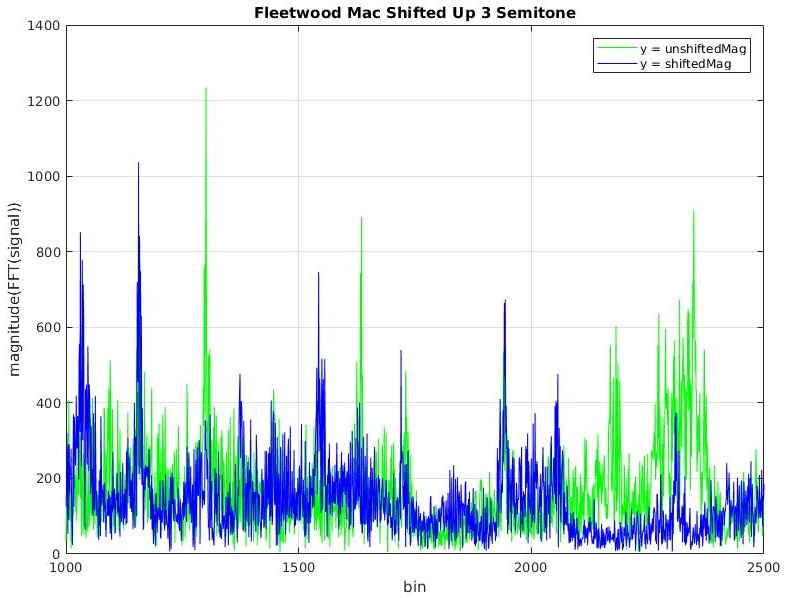
\includegraphics[width=.49\linewidth]{fleet+3zoom.jpg}}
\hfill
\end{figure}

\section{Discussion}
As seen in the results above, the pitch shifting algorithm is very effective for altering the frequency response of a signal. It is reliable and works well with all tested sound files. 

It is unknown what causes the amplitude of the sine wave to increase when shifted upward. On the contrary, the amplitude of the shifted Fleetwood Mac sample appeared to have minimal change. That is an area for investigation and improvement with this algorithm.

\section{Conclusion}
This program performs as intended and is a very useful tool for me. I will continue working on it past the duration of this course, testing the performance with larger input files. In addition, I have used the Sigpack DSP library for other projects, and may compare the performance of the STFT from this algorithm to that from Sigpack. And finally, after further development, this could be put on GitHub or another relevant site as freeware for those that would find it useful.


\pagebreak
\section{References}
Bourne, M. (n.d.). What are the frequencies of music notes? Retrieved December 07, 2017, from \url{https://www.intmath.com/trigonometric-graphs/music.php}

Discrete Fourier Transform. (n.d.). Retrieved December 07, 2017, from \newline \url{http://mathworld.wolfram.com/DiscreteFourierTransform.html}

Stephan Bernsee's Blog. (n.d.). Retrieved December 07, 2017, from \newline	\url{http://blogs.zynaptiq.com/bernsee/pitch-shifting-using-the-ft/}

\end{document}